\documentclass[12pt]{article}
\usepackage{graphicx}
\usepackage{titlesec}
\usepackage{xlop}
\usepackage{url}
\usepackage{subcaption}
\usepackage{geometry}
\graphicspath{ {./images/} }
\usepackage[fleqn]{amsmath}
\usepackage{tikz}
\usepackage{listings}
\usepackage{karnaugh-map}
\geometry{
    a4paper, 
    top=20mm,
    left=20mm,
}
\setlength{\parindent}{4em}
\setlength{\parskip}{1em}
\renewcommand{\baselinestretch}{1.5}

\title{Final Project: ES4 Spring 2021}
\date{5/11/2021}
\author{Ibrahima Barry, WIlly Lin \\ Zach Osman, James Eidson \\ ECE Tufts University}

\titleformat{\section}
    {\normalfont\Large\bfseries}{\thesection}{1em}{}[{\titlerule[1pt]}]

\lstdefinestyle{myListingStyle} 
    {
        basicstyle = \small\ttfamily,
        breaklines = true,
    }

\begin{document}

\maketitle

\begin{flushleft}

\section{Overview}
\begin{center}
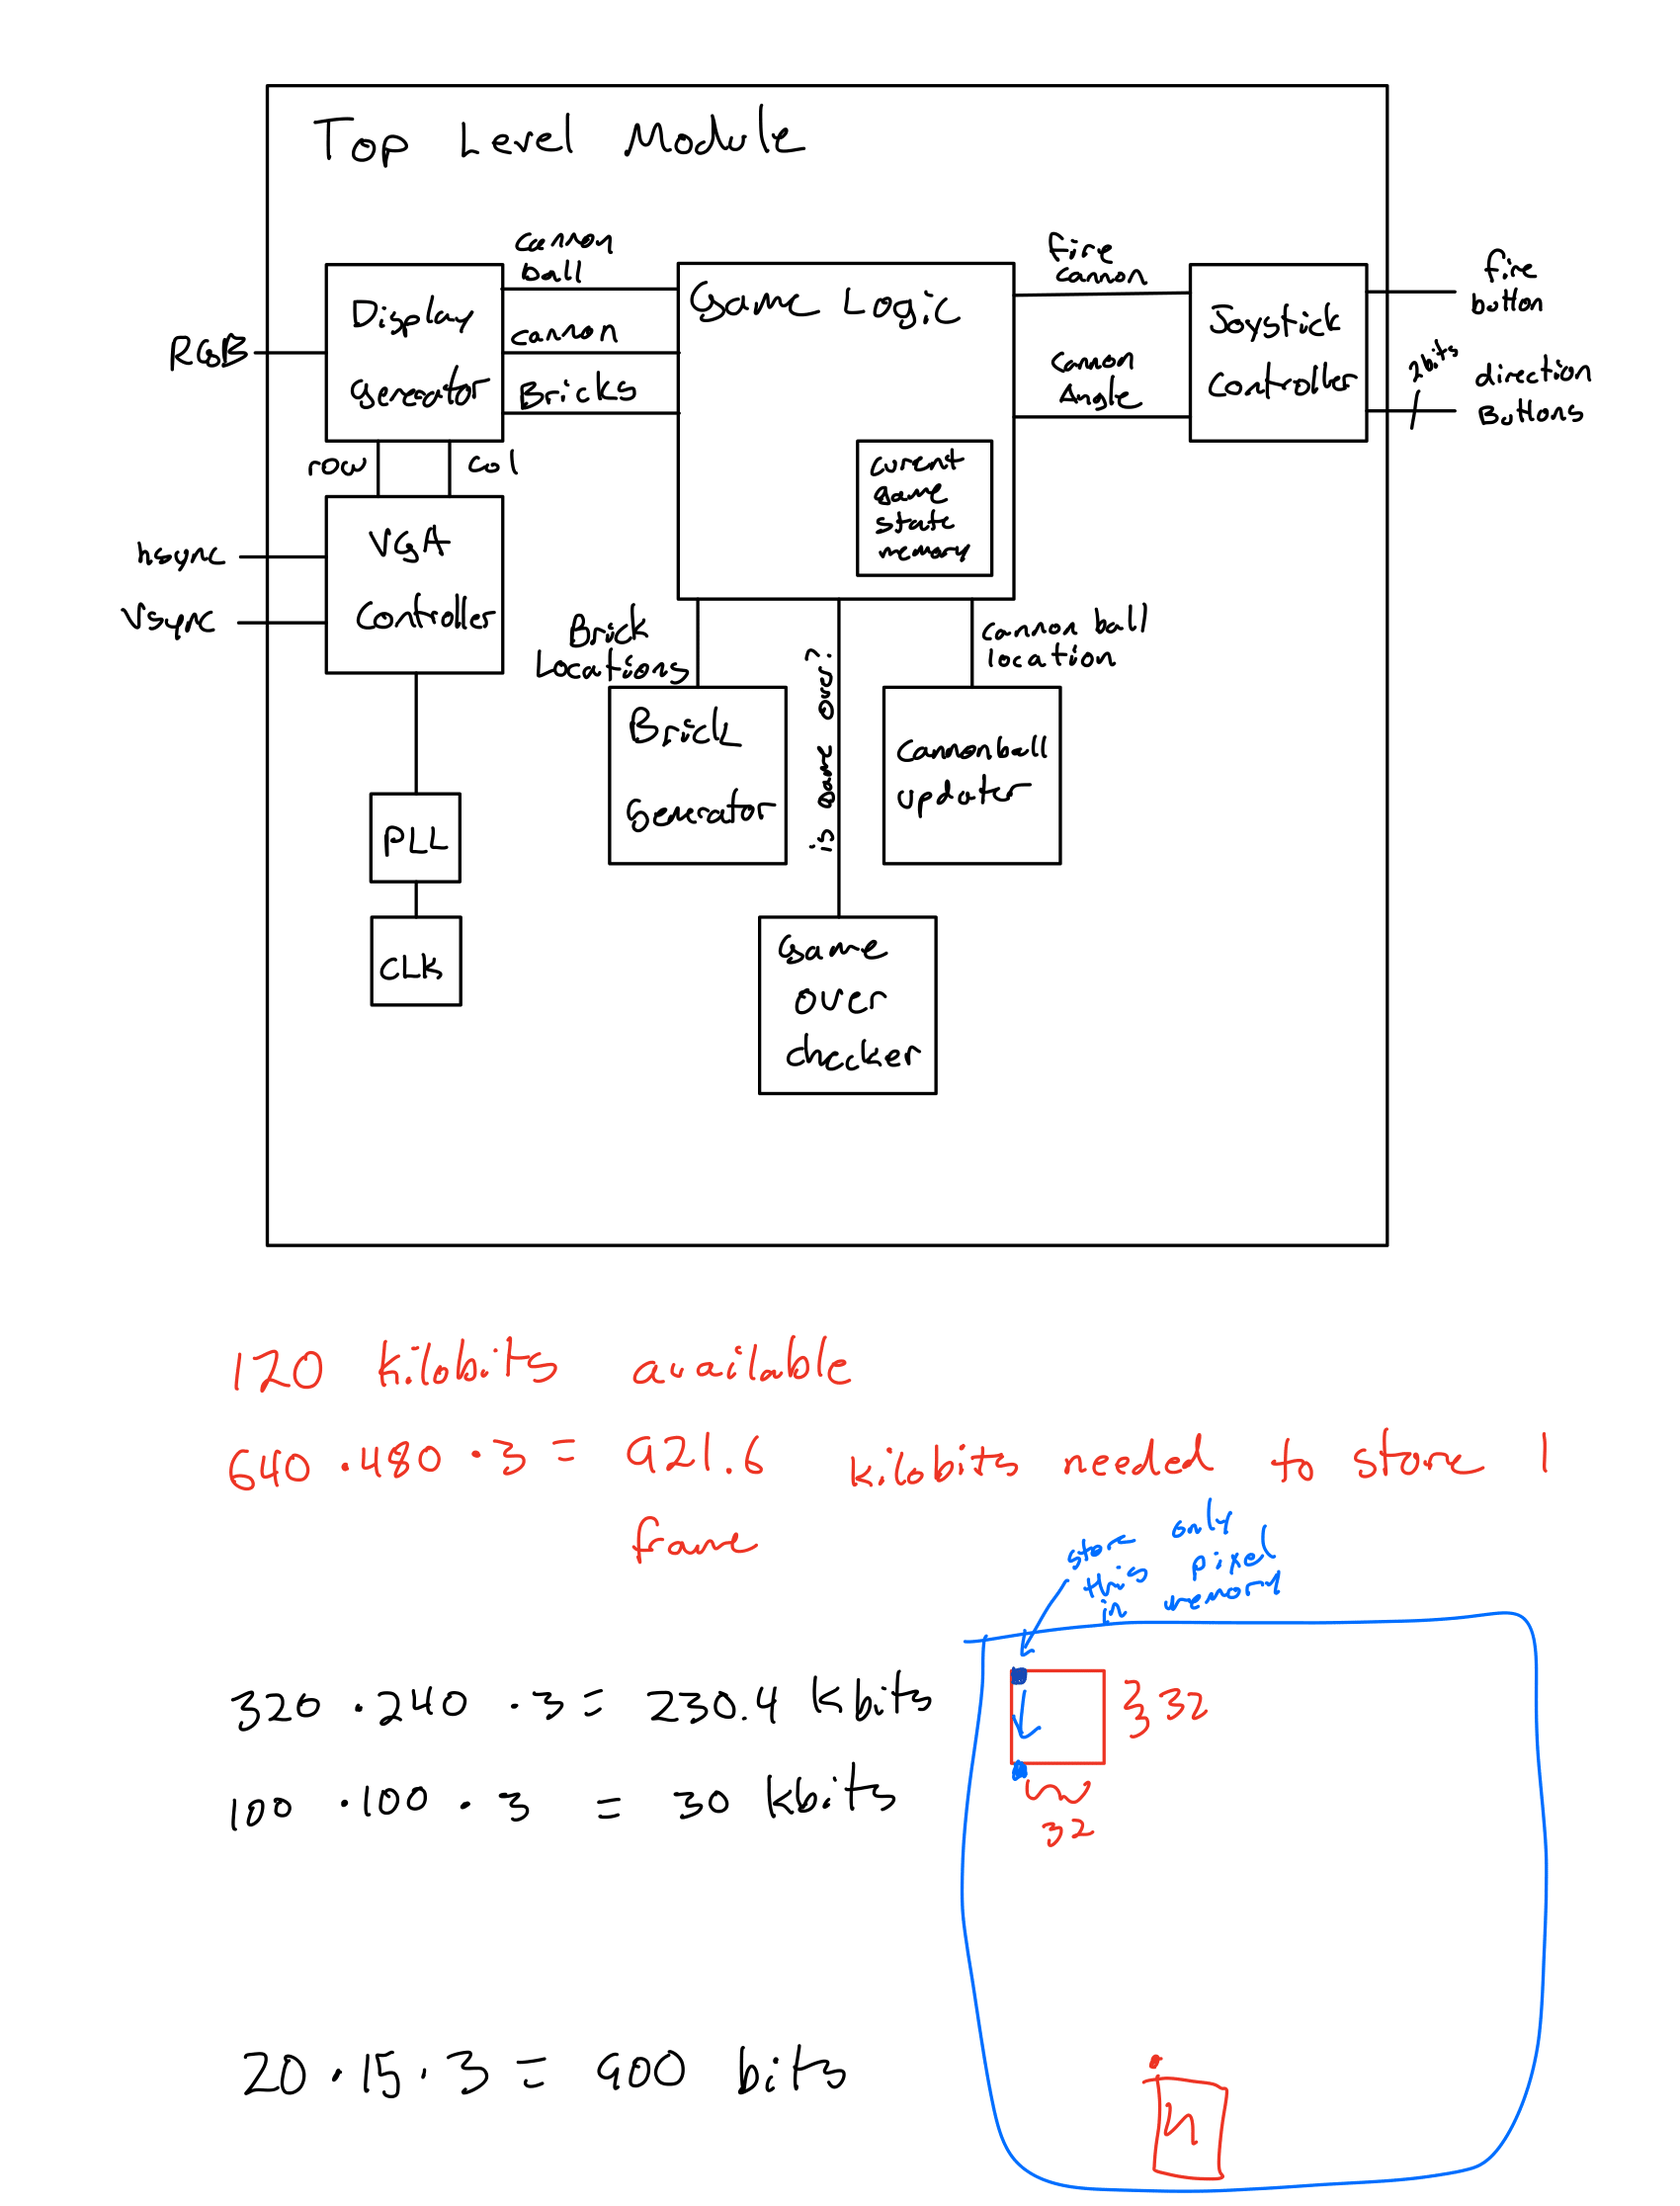
\includegraphics[width=10cm, height=10cm]{blockDiagram}
\end{center}
This game is a variation of the game brickBreaker where the player fires a
cannonball out of a cannon and works to destroy the bricks that are displayed on
the screen. There are three main parts to this project: displays, controls, and
game logic. 'Displays' were done using a VGA, 'controls' were done by using
an NES gamepad, and 'game logic' done in the 'top' module of our project. 
VGA sends the current row and column to display on the screen. The NES gamepad
takes data in the form of buttons pressed and stores it in a shift-register. A
clock is driven for 8 cycles (the number of buttons is 8) and the data signal is
synchronized with the clock. When a button is pressed the corresponding bit of
the output of the register is set to low. The top module controls the general
logic of the game such as drawing the bricks and the cannnon. Top also controls
the memory usage of the game. Overall, objects are drawn in the top module,
displayed via the display module, and those objects are then controlled via the
cannon module (which is connected to the gamepad). 

\section{Technical Description and Design}
\subsection{Top Module}

The top module is where the main game logic is handled. It's inputs are the
12MHz clock of the FPGA and the data from the the controller. It outputs the
necessary signals for the controller and the VGA to work. It's components
are the pll, vga, display, and cannon. The main function of top is to draw the
game objects. This the code to draw the bricks:\\
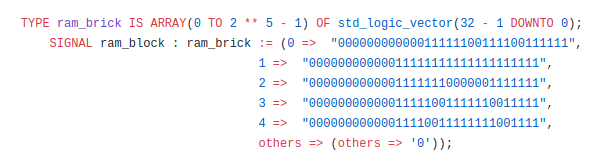
\includegraphics[width=15cm, height=5cm]{drawingBricks}

Where there is a '1' bit is where a brick is drawn. The other details are more
complicated but in general $'1' = $ brick drawn $'0'=$ brick not drawn. $0 - 4$
represent the row being drawin. One of the major challenges encountered here was
figuring out how to destroy a brick when it is hit by a cannon. This means where
there is a $'1'$ bit, meaning a block is drawn at that position, we have to invert
the bit when it is hit by the ball. The display module now knows not to draw
that brick. This was solved by using bit-masking to change the bit.\\ 
eg) consider the row of bricks: $00000000000011111100111100111111$
suppose the block at index 31 needs to be destroyed then the $XOR$ logical
operatoin works well for this. 
$00000000000011111100111100111111 \oplus 00000000000000000000000000000010 =
00000000000011111100111100111101$ 

We create a new bit word of the same size as the ram block  with the corresponding bit we want destroyed to be '1'
and the other bits to '0'. Then $ 1 \oplus 1 = 0$ so this will invert the bit we
want inverted. The other bits are unchanged as $1 \oplus 0 = 1$ and $0 \oplus 0 = 0$.  

\subsection{Display Module}


\section{Results and Testing}

The behavior of the circuit was farily straightforward to test. One could
manually use the DIP switches to do all $2^6$ possible number combinations which
would take very long (but doable). 

Doing this for all possible digits I was sure the circuit functioned correctly.
Also a lab TA looked over my work and agreed it worked as intended.\\

%%%%%%%%%%%%%%%%%%%%%%%%%%%%%%%%%%%%%%%%%%%%%%%%%
% Explain the simuation waves
%%%%%%%%%%%%%%%%%%%%%%%%%%%%%%%%%%%%%%%%%%%%%%%%

\section{Debugging Log}

\begin{enumerate}
    \item A few LEDs on the 7-seg weren't lighting up or they were very dim.
    \begin{itemize} 
        \item Manually setting the LEDs on would work but not otherwise. 
        \item some possible causes included something wrong with VHDL code, the
wiring of the breadboard, and a hardware component not working (not likely). 
        \item Resolution: I needed to ground both GND pins of the Upduino. After
that the dim effect went away. 
        \item Lesson: Always check ground connections because even if other
parts of the circut make sense you can get unexpected results. 
    \end{itemize}
    \item problem: The transistors weren't acting as switches for the LED on the
7-seg. properly. 
    \begin{itemize}
        \item I knew there was a problem because both the digits on the 7-seg
would always have the same numerical value. Both digits were displaying the
value of the ones place. 
        \item possible causes included wiring of the transistor, confusion of
what is the gate, drain and source. 
        \item The issue was that while the transistors were wired correctly they
weren't acting as switches because the power pins of the 7-seg for both digits
were also connected. I.e the transistors weren't controlling the flow of current
in a meaningful way since both the digits were always on regardless of the what
the transistors were doing. 
        \item the lesson I learned was to really understand what each component
does and not just wire it up mindlessly. If I understood the role of the
transistors, I would have recognized that the LED's on the 7-seg do not need to
be connected to power while the source of the transistor was already connected
to power. 
    \end{itemize}
    \item problem: The LEDs weren't giving values as expected from the input
given by the DIP switches. 
        \begin{itemize}
            \item There was a problem because when I toggled the switches the
LEDs weren't producing the correct values. 
            \item Possible causes included: FPGA pin's not connected properly,
the logic in the VHDL code. 
            \item It turned out that the reset signal on my counter was not set
to any value. After making this change the outputs seen on the LEDs of the 7-seg
were correct. 
        \end{itemize}

\end{enumerate}

\section{Reflection} 

\begin{enumerate}
    \item What was the most valuable thing you learned, and why?\\
        - I learned how to debug my VHDL code in a way different to how one
debugs code in a language like Java or Python. Many times the code can compile
but the hardware implementation may not behave the way you want it.
    \item What skills or concepts are you still struggling with? What will you do to 
          learn or practice these?\\
        - I'm still struggling with how to write testbenches for very large
complicated code. To practice I will review the textbook and try writing
testbenches for other VHDL code I've written. 
    \item This assignment took about 72 hours (not including several hours
tyring to write a testbench) during all of the  days in which I
worked on it. 

\end{enumerate}

\section{Work Divison} 

\section{source code}
%Add link to the github


\end{flushleft}
\end{document}
